\documentclass{beamer} %% normal document
%\documentclass[notes]{beamer} %% notes in normal document
%\documentclass[draft,notes]{beamer} %% draft with notes
%\documentclass[handout]{beamer} %% handout

\usepackage{fontspec, unicode-math, caption}
\usepackage[ngerman]{babel}
\usepackage{graphicx}
\usepackage{float}

%% usefull for handout with blank lines
%\usepackage{handoutWithNotes}
%\pgfpagesuselayout{2 on 1 with notes}[a4paper,border shrink=5mm]

%% usefull for presentation
%\setbeameroption{show notes on secondscreen=left}

\definecolor{bettergreen}{rgb}{.1,.7,.1}

\usetheme{Dresden}
\usecolortheme[named=bettergreen]{structure}
\useoutertheme{split}
\setbeamertemplate{caption}[numbered]
\captionsetup{labelformat=simple,font=scriptsize,labelfont=scriptsize}

% puts Frame numbers in Dresden template
\newcommand*\oldmacro{}%
\let\oldmacro\insertshorttitle%
\renewcommand*\insertshorttitle{%
	\oldmacro\hfill%
	\insertframenumber\,/\,\inserttotalframenumber}

\title[]{}

\author{
	Johannes Visintini, Philip Bell,\\
	Moritz Nöltner
}

\institute[IFI]{
	Vorlesung: Einführung in Software Engineering\\
	Institut für Informatik\\
	Universität Heidelberg
}
 
\begin{document}

	\begin{frame}
		\titlepage
		\note{ }
	\end{frame}

	\section{Klassendiagramm}

	\begin{frame}{Klassendiagramm}
		\begin{figure}[H] %% There is no sense in having this image appear somewhere else
			\centering
			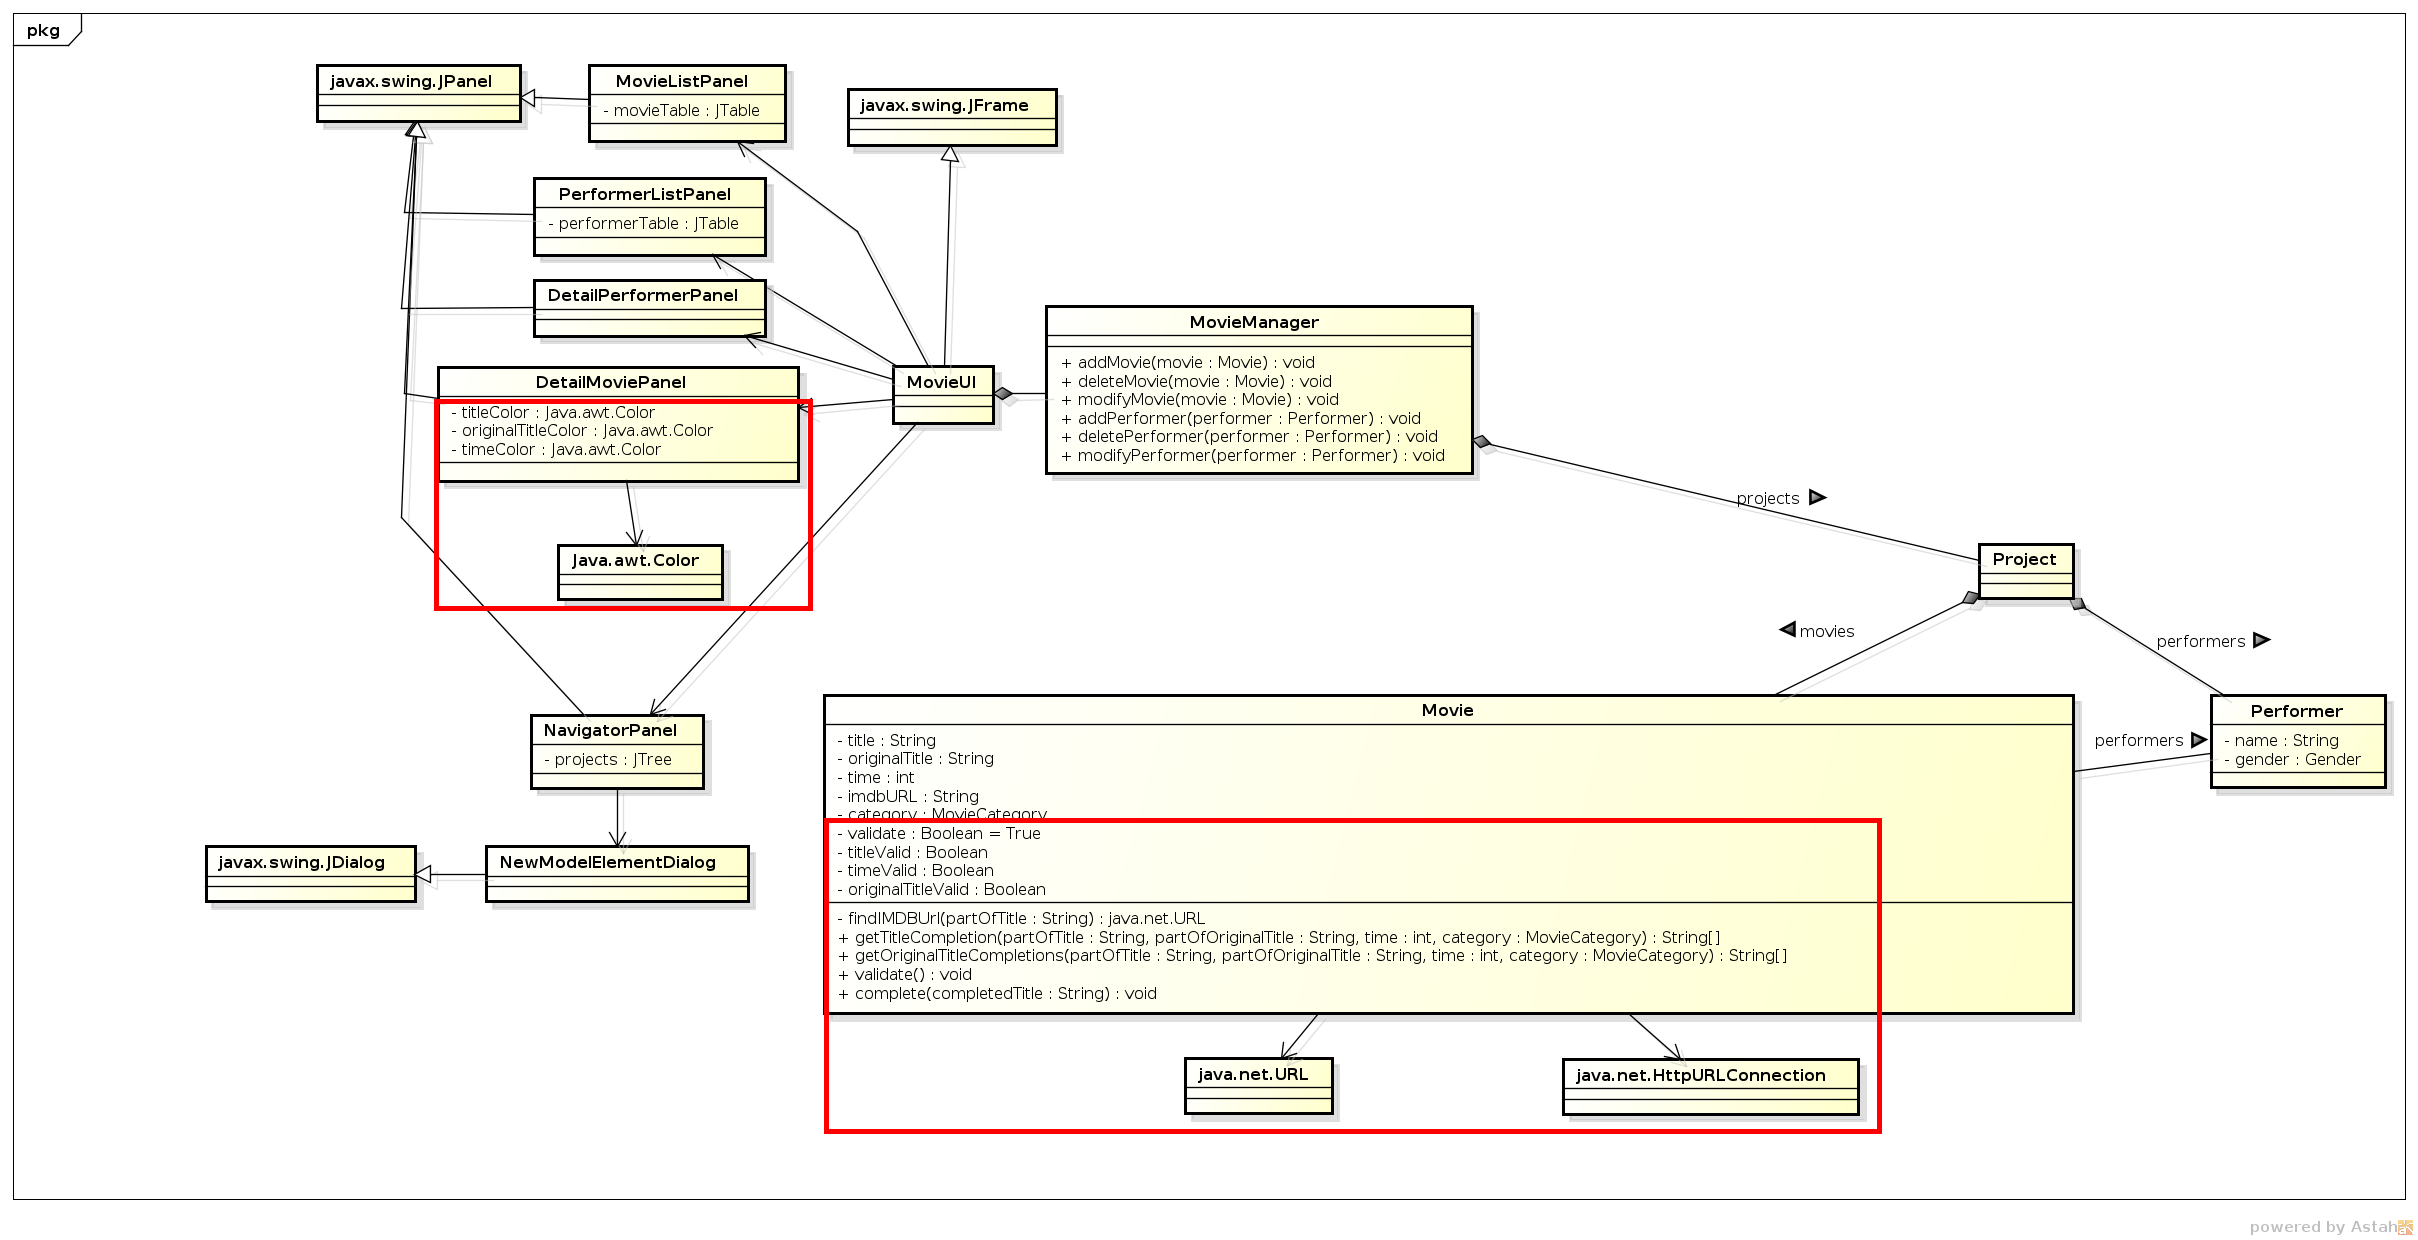
\includegraphics[width=\linewidth]{klassendiagramm2.png}
		\end{figure}
	\end{frame}

	\section{Sequenzdiagramme}
	\subsection{changeTitle}
	\begin{frame}{Sequenzdiagramme - changeTitle}
		\begin{figure}[H] %% There is no sense in having this image appear somewhere else
			\centering
			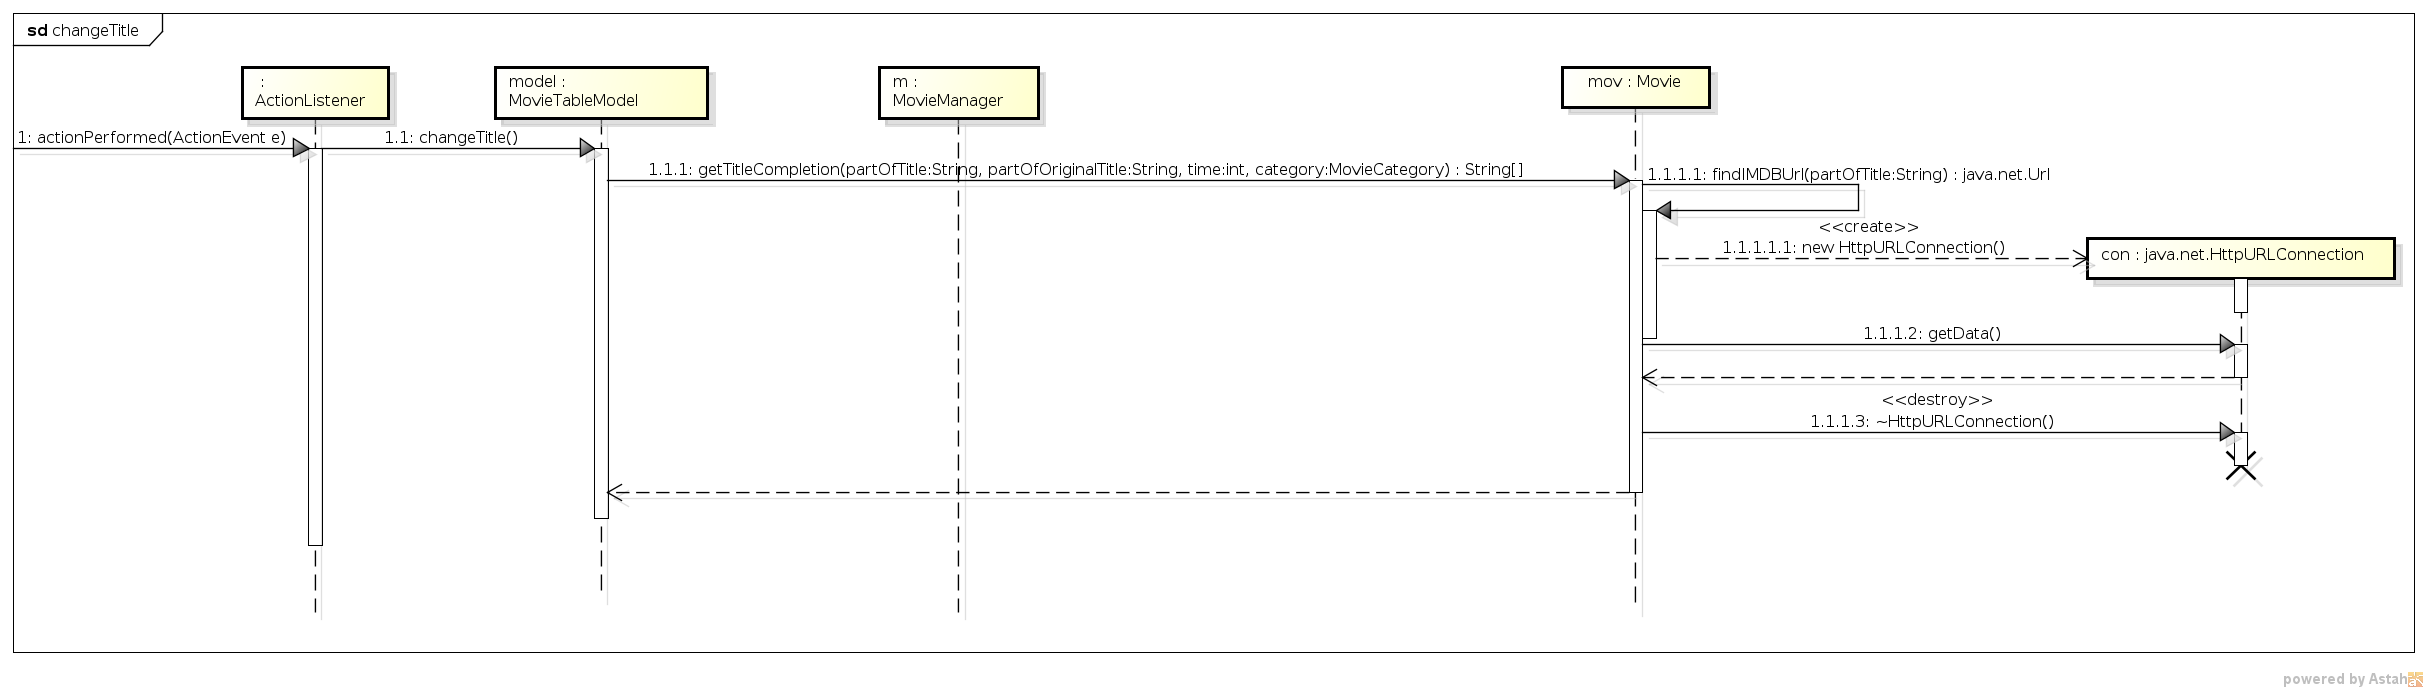
\includegraphics[width=\linewidth]{changeTitle.png}
		\end{figure}
	\end{frame}

	\subsection{clickOnProposedTitle}
	\begin{frame}{Sequenzdiagramme - clickOnProposedTitle}
		\begin{figure}[H] %% There is no sense in having this image appear somewhere else
			\centering
			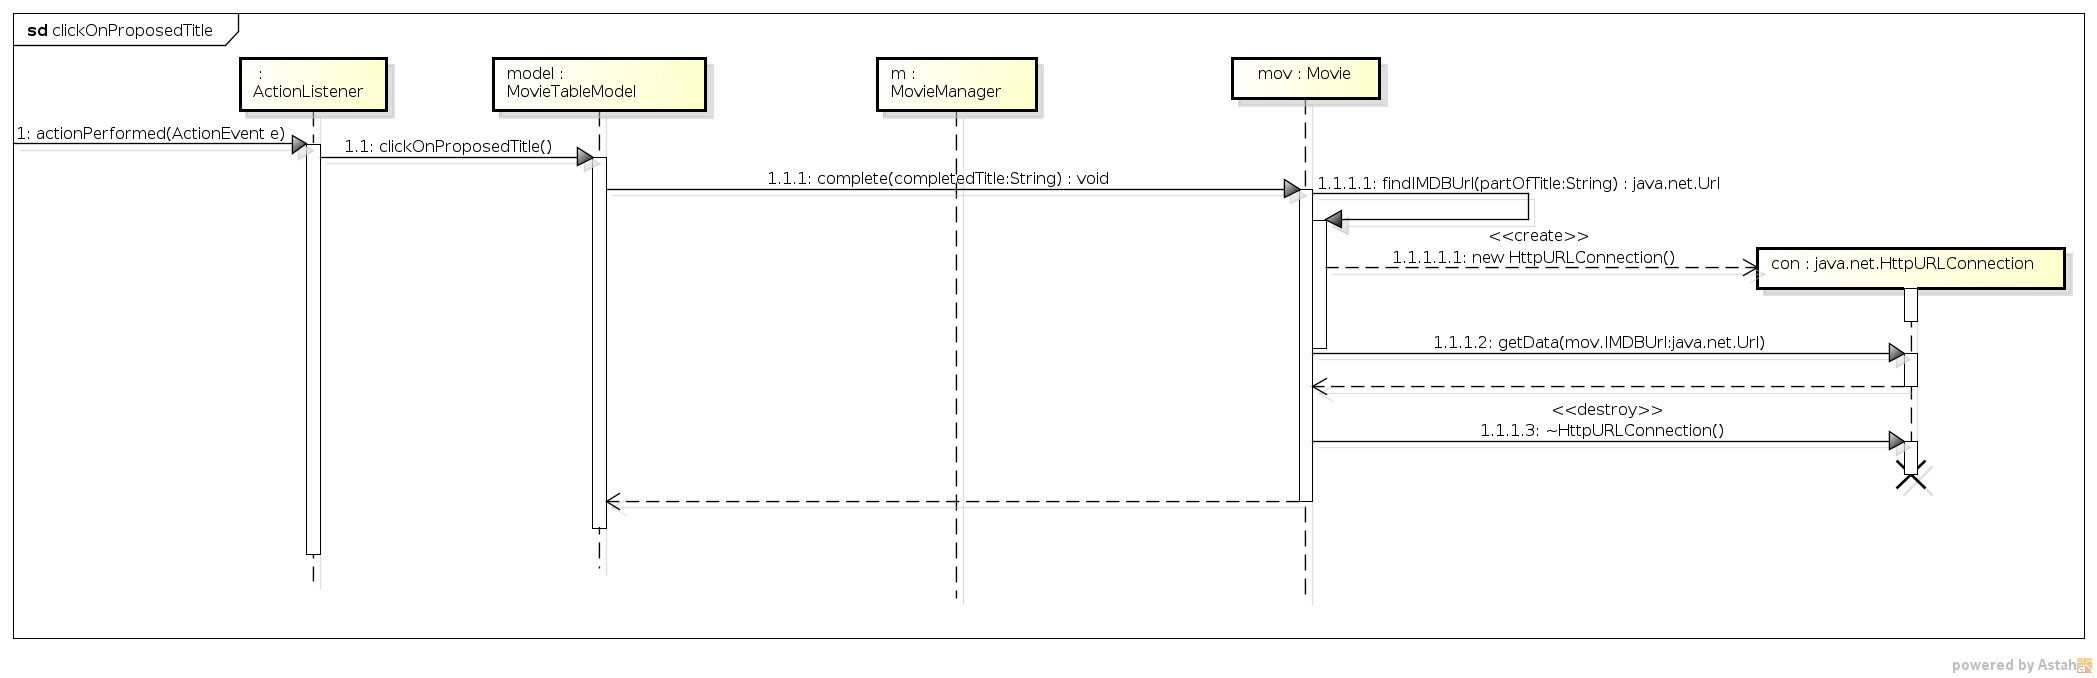
\includegraphics[width=\linewidth]{clickOnProposedTitle.png}
		\end{figure}
	\end{frame}

	\subsection{set<MovieAttribut>}
	\begin{frame}{Sequenzdiagramme - set<MovieAttribut>}
		\begin{figure}[H] %% There is no sense in having this image appear somewhere else
			\centering
			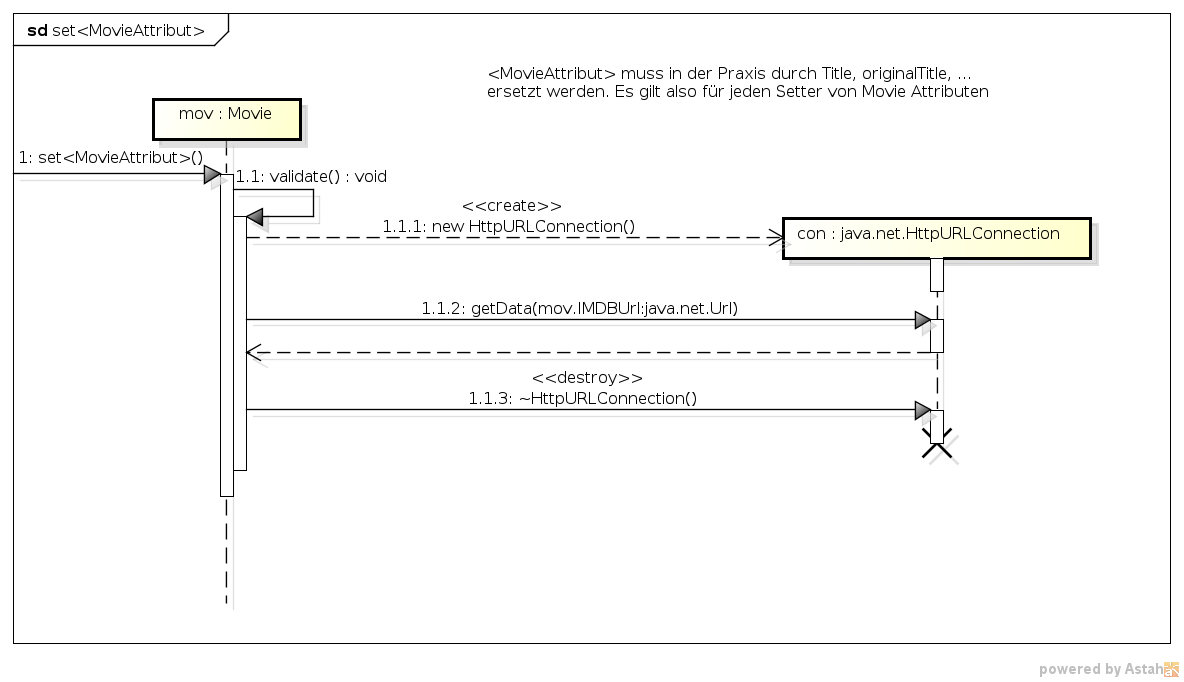
\includegraphics[width=\linewidth]{set_MovieAttribut_.png}
		\end{figure}
	\end{frame}

	\section{Begründung}
	\begin{frame}{Begründung}
		\begin{itemize}
			\item optimale Nutzerfreundlichkeit durch direktes visuelles Feedback
			\item Vermeidung von weiteren Interfaces und Overviews
			\item Implementierung direkt in die Movie Klasse\\
				→ keine unnötigen Klassen\\
				→ Schlankere Implementation
		\end{itemize}
	\end{frame}

	\section{}
	\begin{frame}
		\center{\Huge ENDE}
	\end{frame}

\end{document}
